% !TEX TS-program = lualatex
% !TEX encoding = UTF-8

% This is a simple template for a LuaLaTeX document using gregorio scores.

\documentclass[letterpaper,12pt]{book} % use larger type; default would be 10pt

\input{header.inc}

\geometry{letterpaper,outer=0.4in,inner=0.9in,top=0.6in,bottom=0.8in}

\begin{document}

\printsmalltitle{Audi Benigne Conditor}

\garamondbig
\greannotation{Hymn.}
\greannotation{2.}
\gregorioscore{231_hy--audi_benigne_conditor--solesmes}

\bigskip

\printsmalltitle{Vexilla Regis}

\greannotation{Hymn.}
\greannotation{1.}
\gregorioscore{232_hy--vexilla_regis_prodeunt--solesmes}

\bigskip

\begin{centering}
\vfill

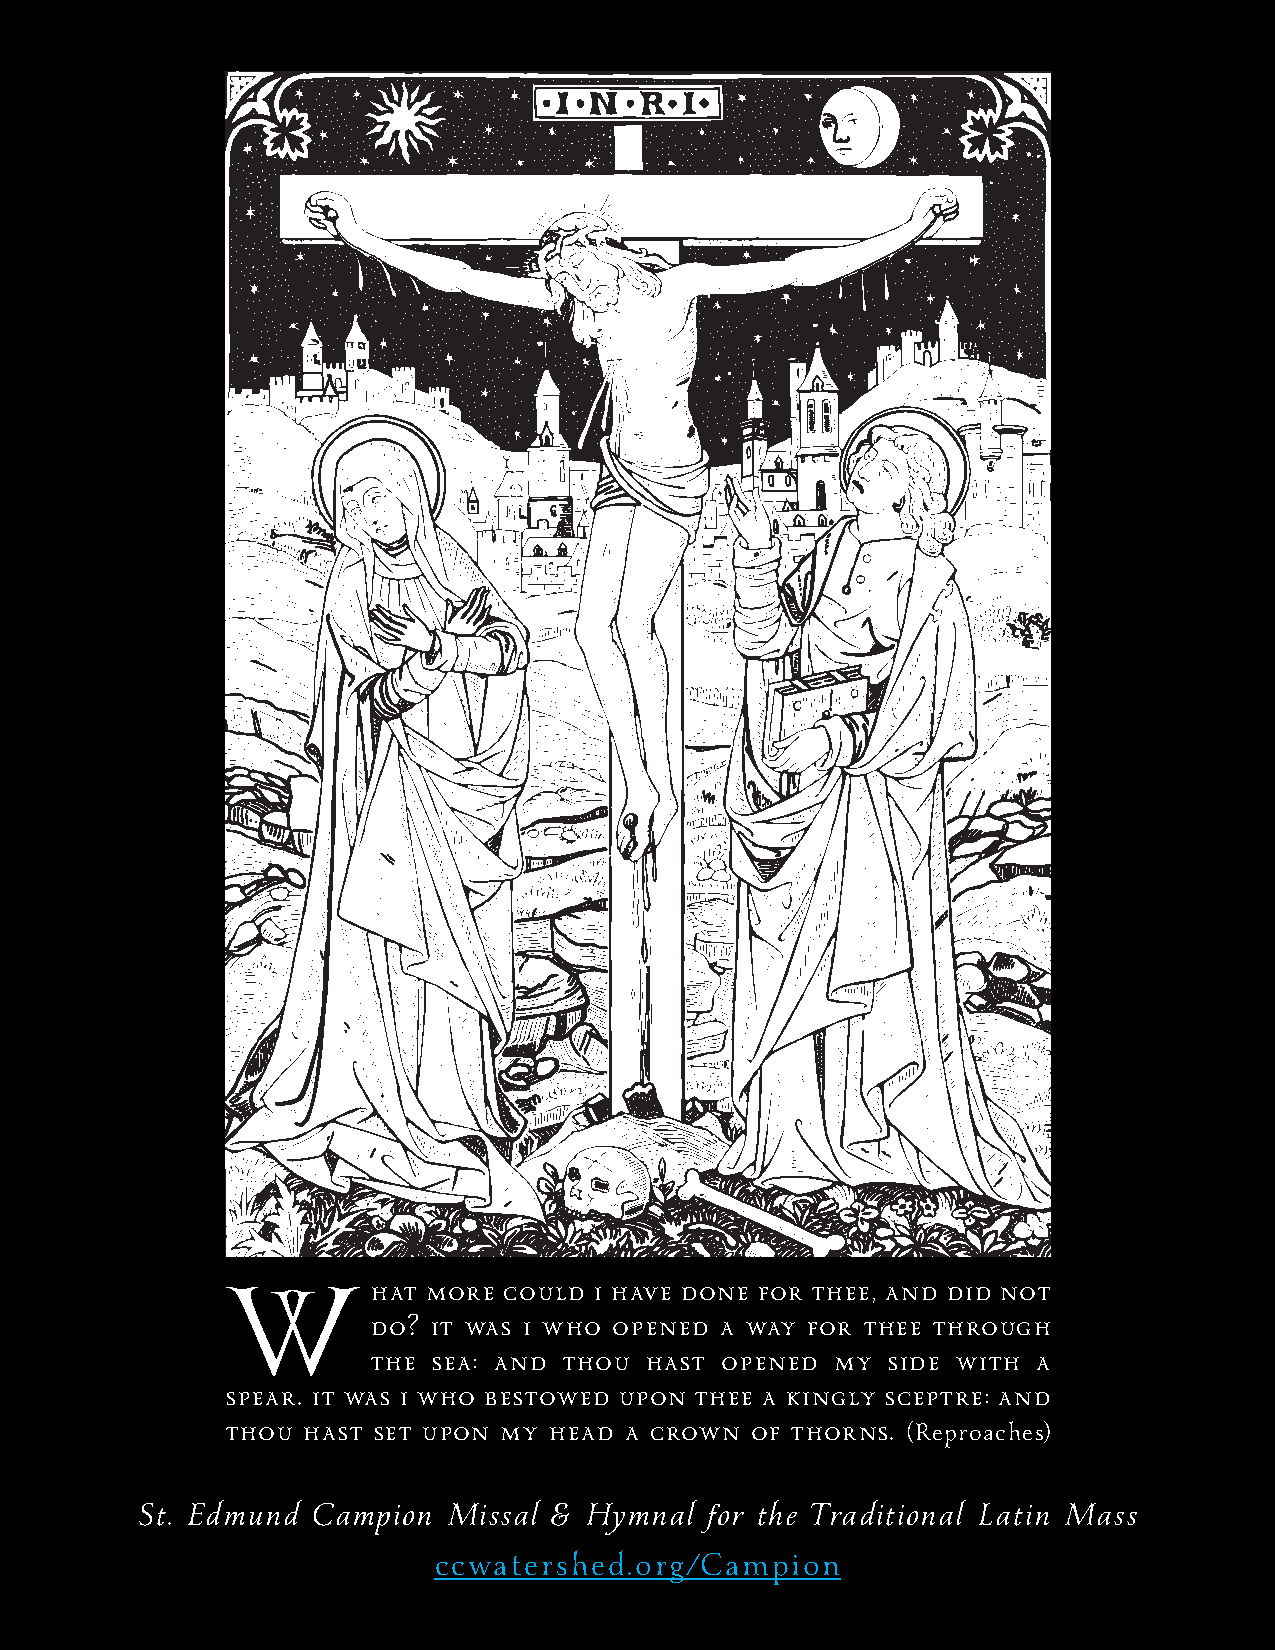
\includegraphics[clip,trim=1.49in 2.604in 1.48in 0.455in,height=6.9in]{../234_17-49-36_0.pdf}

\vfill

\end{centering}


\end{document}